\documentclass[a4paper, 12pt]{article}
\usepackage{amssymb}
\usepackage{amsmath}
\usepackage{verbatim}
\setcounter{tocdepth}{3}
\usepackage{graphicx}
\usepackage{afterpage}
\usepackage{floatpag}
\floatpagestyle{empty}
%\usepackage[a4paper, total={4in, 6in},margin=4in]{geometry}
\usepackage[export]{adjustbox}
%\usepackage[paperwidth=7.0in, paperheight=10.7in]{geometry}
%\usepackage{layout}
%\layout{layoutwidth=180mm,layoutheight=227mm}
%\geometry{a4paper,left=25mm,right=25mm,top=25mm,bottom=25mm,heightrounded}
%\usepackage[a4paper]{geometry}
\usepackage{listings}
\usepackage{subfigure}
\usepackage{wrapfig}
\usepackage[hyperindex=false,colorlinks=false]{hyperref}
\usepackage{fullpage}
\usepackage{tikz}
\usetikzlibrary{shapes.geometric, arrows}
\DeclareMathSizes{20}{20}{20}{20}

\tikzstyle{startstop}=[rectangle, rounded corners, minimum width=3cm, minimum height=1cm, text centered, text width=4cm, draw=black,fill=red!30]

\tikzstyle{io}=[trapezium, trapezium left angle=70, trapezium right angle=110, minimum width=3cm, minimum height=1cm, text centered, text width=4cm, draw=black, fill=blue!30]

\tikzstyle{process}=[rectangle, minimum width=3cm, minimum height=1cm, text centered, text width=4cm, draw=black,fill=orange!30]

\tikzstyle{decision}=[diamond, minimum width=3cm, minimum height=1cm, text centered, text width=4cm, draw=black, fill=green!30]

\tikzstyle{arrow}=[thick,->,>=stealth]

\begin{document}

\begin{titlepage}

%\newcommand{\HRule}{\rule{\linewidth}{0.5mm}} % Defines a new command for the horizontal lines, change thickness here
\newcommand{\HRule}{\rule{135mm}{0.5mm}} % Defines a new command for the horizontal lines, change thickness here

\center % Center everything on the page

%----------------------------------------------------------------------------------------
%   HEADING SECTIONS
%----------------------------------------------------------------------------------------

\textsc{\LARGE Technische Universit{\"a}t M{\"u}nchen}\\[1.5cm] % Name of your university/college
\textsc{\Large Chair For Logistics and Supply Chain Management}\\[0.5cm] % Major heading such as course name

%----------------------------------------------------------------------------------------
%   TITLE SECTION
%----------------------------------------------------------------------------------------
\vspace{48mm}
\HRule \\[0.4cm]
{ \Large \bfseries Implementation of a Metaheuristic\\for the\\Discrete Network Design Problem}\\[0.5cm] % Title of your document
\HRule \\[1.5cm]

%----------------------------------------------------------------------------------------
%   AUTHOR SECTION
%----------------------------------------------------------------------------------------
\vspace{48mm}
\begin{minipage}{0.4\textwidth}
\begin{flushleft} \large
\emph{Student:}\\
Nishanth Nagendra % Your name
\end{flushleft}
\end{minipage}
\begin{minipage}{0.4\textwidth} 
\begin{flushright} \large
\emph{Supervisor:} \\
Prof. Dr. Stefan Minner \\~\\ % Supervisor's Name
\emph{Advisor:} \\
Dipl.-Math. Pirmin Fontaine % Advisor's Name
\end{flushright}
\end{minipage}\\[2cm]

% If you don't want a supervisor, uncomment the two lines below and remove the section above
%\Large \emph{Author:}\\
%John \textsc{Smith}\\[3cm] % Your name

%----------------------------------------------------------------------------------------
%   DATE SECTION
%----------------------------------------------------------------------------------------

{\large \today}\\[2cm] % Date, change the \today to a set date if you want to be precise

\end{titlepage}

\begin{center}
\huge \bfseries Acknowledgement
\end{center}
\thispagestyle{empty}
\vspace{35mm}
I would like to thank Mr. Fontaine for his constant support and guidance throughout the project especially when I faced some challenges in understanding certain topics. I would also like to thank Prof. Dr. Stefan Minner for providing me with this opportunity to work on such an Inter-Disciplinary project.

\newpage

\begin{center}
\huge \bfseries Abstract
\end{center}
\thispagestyle{empty}
\vspace{35mm}

The field of transportation planning involves a large class of problems that are characterized by multiple levels of decision making. Examples include selection of links for capacity improvements(network design), toll setting, traffic signal setting etc. In each of these problems, government or industry officials make one set of decisions to improve the network performance and at another level users make choices with regard to route, origin-destination etc. The discrete network design problem(DNDP) is one such problem which deals with the selection of link additions to an existing road network, with given demand from each origin to destination. The objective is to make an optimal investment decision to minimize the total travel cost in the network, while accounting for the route choice behavior of network users. This optimization problem is recognized to be NP hard because it is computationally difficult due to its non convexity owing to the bilevel nature and non-linear objective functions in most of the real cases. Finding exact or globally optimum solutions for such problems is very difficult. In mathematical optimization, a metaheuristic is a general high level procedure that can be quickly applied to different kinds of problems to provide a sufficiently good solution especially when there is limited computation capacity. These techniques sample a set of solutions which is too large to be completely sampled. Genetic algorithm is one such kind of a metaheuristic which tries to imitate the evolution of population by starting with a random set of candidate solutions that is evolved towards better solutions. The aim of the project is to implement this metaheuristic on the DNDP and to experiment with small to large size datasets(networks) widely mentioned in the literature to derive empirical results and to conclude on the effectiveness, solvability and quality of solutions obtained.

\newpage
\thispagestyle{empty}
\tableofcontents
\newpage

\setcounter{page}{1}
\section{Introduction}
The network design problem(NDP) is concerned with the modification of a transport infrastructure by adding new links or improving existing ones. In most applications, one is interested in selecting from among a relatively small set of improvements to an existing network rather than designing an entirely new network from scratch. Network design problems arise in many transportation modes: urban mass transit, highway, rail etc. Most applications have been in highway improvement, however. The discrete network design problem(DNDP) deals with the selection of link additions to an existing road network, with given demand from each origin to destination. The objective is to make an optimal investment decision in order to minimize the total travel cost in the network, while accounting for the route choice behavior of network users. Another form of this problem is the continuous network design problem(CNDP) which deals with the optimal capacity expansion of existing links.\par
\noindent
\\These combinatorial problems are recognized as NP Hard due to the considerable amount of computational difficulties faced in trying to solve them because of their non-convex nature and due to the form of a bi-level mixed integer program with a large number of 0-1 variables. This Inter disciplinary project deals with only the discrete form of the NDP and considers the following kind of problem which often arises in transportation planning: minimize total travel expenditure subject to a budget constraint on the total construction cost of new links.
 
\subsection{Problem Formulation}
Bilevel problems are mathematical programming problems consisting of a special kind of optimization where one problem is embedded within another. The outer optimization task is commonly referred to as the upper level(or the leader) optimization task with a nested optimization problem(the lower one - also called follower) in the constraints. First, the leader has to decide over a subset of the decision variables which effects the objective value of the follower. Afterwards, the follower has to decide over the other subset of decision variables, which affects the objective value of the leader. The problem we are considering to solve here is a bilevel linear program with binary leader variables and continuous follower variables. An application of bilevel programming is network design problems where the objective of the network designer is to reduce congestion in the network and the objective of the follower is to find the fastest way from origin to destination. Existing methods for solving this problem can be roughly divided into the following categories:\par
\begin{itemize}
\item Methods based on vertex enumeration
\item Methods based on kuhn tucker conditions
\item Fuzzy approach
\item Methods based on meta heuristics
\end{itemize}

%\begin{figure}[htbp]\centering
%
\includegraphics{./try.eps}
%\caption{Trial}
%\label{fig 1}
%\end{figure}
%\epsfbox{./try.eps}

\subsection{InterDisciplinary Project}
The implementation of this project required knowledge of C/C++ programming, Data Structures, linear programming concepts, usage of the C++ BCL(Builder component library) provided by a commercially well known optimization suite called FICO Xpress. The application of these technologies is for a well known real world problem like DNDP observed in transportation science resulted in this project to be of Inter-Disciplinary nature. As a part of the preparation for implementing this project, a good amount of knowledge on \textbf{metaheuristics} and \textbf{DNDP} was acquired from the course \textbf{"TRANSPORTATION LOGISTICS"} offered by the \textbf{CHAIR OF LOGISTICS AND SUPPLY CHAIN MANAGEMENT.}\par
\noindent
\\
The objective of this course was to get an overview of the modeling techniques, exact as well as heuristic search methods tailored to the different transportation problems studied. The course consisted of a sequence of lectures, exercise classes and case studies. It also deals on how to model and analyze transportation problems using quantitative methods. It covers many of the real world problems observed in Transportation Planning such as Traveling Salesman Problem(TSP), Vehicle Routing Problems(VRP), Network Flow Problems, Inventory Routing etc. and techniques such as Metaheuristics used to solve them.\par
\begin{itemize}
\item \textbf{Transportation Problems}: Linear programming formulations, Solving methods like Northwest corner rule, Column minimum rule, Matrix minimum rule, MODI(Modified Distribution) method, Extensions to Transshipment problem and several others.
\item \textbf{Traveling Salesman Problem}: TSP models(Symmetric and Asymmetric), Exact solution methods, Heuristics like nearest neighbor and r-opt method, Arc Routing problem.
\item \textbf{Vehicle Routing Problem}: Different modeling schemes for VRP using Linear programming formulations, Sweep method, Savings method as solution techniques for VRP problems, Extensions of VRP and Savings method.
\item \textbf{Inventory Routing Problem}: Lot-Sizing Problem, Inventory Routing Problem(IRP)
\item \textbf{Transportation planning in networks}: Dynamic optimization, Hub-Spoke systems, Shortest path problem, dijkstra's algorithm, Minimum spanning tree problem, Maximum flow problem.
\item \textbf{Metaheuristics}: Basics of metaheuristics, Simulated Annealing with TSP as its case study, Tabu Search, Genetic Algorithm and its application to TSP as a case study, Application of metaheuristic on VRP.
\item \textbf{Traffic Network Design Problems}: Covers Traffic assignment problem(TAP), Extensions of TAP like Discrete Network Design Problem(DNDP), Line planning.
\item \textbf{Revenue Management}: Segmentation, Price differentiation, Models of Overbooking.
\item \textbf{Packing logistics}: Fundamentals of Packing and its stages, Cutting Stock Problem, Knapsack Problem, Bin Packing Problem.
\item \textbf{Container Shipping and Terminals}: Working of container terminals, Job-Shop and Flow-Shop Problems, Branch and Bound method, Usage of Gantt-Chart.
\item Most of the above mentioned problems studied in transportation planning involved modeling them using Linear Programming and looking at their solving methods.
\end{itemize}
The course gave an introduction to many of the important problems observed in transportation science one of which is DNDP that the IDP deals with specifically. In relevance to the project, the course dealt with the necessary topics such as different kinds of metaheuristics, their algorithms followed by case studies and numerical problems to better understand these techniques. The bilevel formulation of DNDP was also introduced with TAP as its nested optimization problem and some of the techniques to solve them exactly or approximately.\par
\noindent
\\
A rough \textbf{timeline} from when the project started till its anticipated completion time is given below.
\begin{itemize}
\item Dec 2014 - Start of IDP with initial literature survey but main focus on the course.
\item Feb 4, 2015 - Completion of the exam on the course \textbf{"TRANSPORTATION LOGISTICS"}.
\item Feb 4, 2015 to April 14, 2015 - Further literature reading, setup, understanding and practical usage of the FICO Xpress software, learning to write code using BCL component.
\item April 15, 2015 to July 31, 2015 - Implementation phase with good amount of testing. Further testing will follow on larger datasets with additional code to provide extensions.
\item Aug 1, 2015 to Aug 30, 2015 - Documentation and Presentation
\item Early Sep 2015 - Completion of IDP
\end{itemize}

\subsection{Software Requirements}
The project has been implemented in C with the help of an API(Linux version) provided by a commercial software suite for C++.\\~\\
\textbf{\boldmath$FICO^{TM}$ Xpress Optimization Suite:}   FICO Xpress Optimization Suite is a sophisticated mathematical modeling and optimization software. Its tools enable operational research and management professionals, analysts, and consultants to rapidly develop optimization applications that solve complex, real-world business and customer engagement challenges. It provides easy ways to create, deploy and utilize business optimization solutions based on scalable high-performance algorithms, a flexible modeling environment and rapid application and reporting capabilities.\\~\\
Optimization problems have to be solved computationally to good approximation and require the usage of sophisticated optimization 
softwares that can provide a library(API- Application programming interface) for the programmer to do the same. The programmer can use this to
 implement an application demonstrating the solving methods for DNDP. This is first done by modeling the DNDP in the form of a bilevel mixed 
integer linear program via the API provided by FICO Xpress BCL component and using its optimization modules to solve the nested optimization 
problem of TAP.\par                   
\begin{figure}[h]
\centering
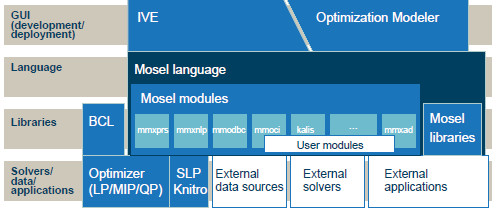
\includegraphics[width=0.65\textwidth, clip]{./Xpress.jpg}
\vspace{-0.15in}
\caption{Xpress product suite}
\label{fig:1}
\end{figure}
\noindent
\textbf{Libraries for embedding:}   An option available from this software for embedding mathematical models into large applications is by developing a model directly in a programming language with the help of a model builder library \textit{Xpresss-BCL}. BCL(Builder Component Library) allows a user to formulate models with objects(decision variables, constraints, index sets) similar to those of a dedicated modeling language. All libraries are available for C, C++, Java, C\#, and Visual Basic(VB). For this project we will be using the library for C++.\\ \par
\noindent
The Xpress-BCL Builder Component Library(BCL) provides an environment in which the Xpress user may readily formulate and solve linear, mixed integer and quadratic programming models. Using BCL’s extensive collection of functions, complicated models may be swiftly and simply constructed, preparing problems for optimization. Not merely limited to specific model construction, however, BCL’s flexibility makes it the ideal engine 
for embedding in custom applications for the construction of generic modeling software. In combination with the Xpress-Optimizer, the two form 
a powerful combination.\\ \par
\noindent
Model formulation using Xpress-BCL is constraint-oriented. Such constraints may be built up either coefficient-wise, incrementally adding 
linear or quadratic terms until the constraint is complete, or through use of arrays of variables, constructing the constraint through a 
scalar product of variable and coefficient arrays. The former method allows for easier modification of models once constructed, whilst the 
latter enables swifter construction of new constraints. To complement the model construction routines, BCL supports a number of functions which allow a completed model to be passed directly to the Xpress-Optimizer, solved by the optimizer, and solution information reported back 
directly from BCL.
\newpage
\section{Modeling}
\subsection{Traffic Assignment Problem}
\vspace{5mm}
\begin{large}\textbf{Definitions:}\end{large}
\begin{itemize}
\item Set of Nodes \textit{N}
\item Set of links A with
\begin{itemize}
\item capacity $c_{a}$
\item congestion factor $B_{a}$
\item free flow travel time $T_{a}$
\end{itemize}
\item Set of origins $R\ \subseteq\ N$ and destination $S\ \subseteq\ N$ with demand $q_{rs}$ 
\end{itemize}
\begin{large}\textbf{Decision variables:}\end{large}
\begin{itemize}
\item $x_{a}$ travelers on link a
\item ${f_{a}}^{rs}$ travelers of OD-pair (r,s) on link a
\end{itemize}
\begin{large}\textbf{Constraints:}\end{large}\\
Travel time function on link a: 
\begin{large}
\boldmath\begin{equation*}
t_{a}\left(x\right) = T_{a}\left(1+B_{a}\left(\frac{x}{c_a}\right)^4\right)
\end{equation*}
\end{large}
Objective:
\begin{large}
\boldmath\begin{equation*}
\mathrm{min}\sum_{a\in{A}} \int\limits_{0}^{x_a}t_{a}\left(x\right)dx = \mathrm{min}\sum_{a\in{A}}\left(T_{a}B_{a}+\frac{T_{a}x_{a}}{5{c_{a}}^4}{x_{a}}^5\right) 
\end{equation*}
\end{large}
Demand at origin: 
\begin{large}
\boldmath\begin{equation*}
\sum_{j\in{N}} f_{rj}^{rs} = q_{rs}\  \wedge \ \sum_{j\in{N}} {f_{jr}}^{rs} = 0 \ \ \ \ \mathrm{\forall{r}\in{R},\forall{s}\in{S}} 
\end{equation*}
\end{large}
Demand at destination: 
\begin{large}
\boldmath\begin{equation*}
\sum_{i\in{N}} f_{is}^{rs} = q_{rs}\  \wedge \ \sum_{i\in{N}} {f_{si}}^{rs} = 0 \ \ \ \ \mathrm{\forall{r}\in{R},\forall{s}\in{S}} 
\end{equation*}
\end{large}
Flow conservation: 
\begin{large}
\boldmath\begin{equation*}
\sum_{i\in{N}} f_{ik}^{rs} = \sum_{j\in{N}} {f_{kj}}^{rs} \ \ \ \ \mathrm{\forall{r}\in{R},\forall{s}\in{S},{k}\in{N}{\backslash}{\{}r,s{\}}}
\end{equation*}
\end{large}
Flow aggregation: 
\begin{large}
\boldmath\begin{equation*}
x_{a} = \sum_{r\in{R},s\in{S}} {f_{a}}^{rs} \ \ \ \ \mathrm{\forall{a}\in{A}}
\end{equation*}
\end{large}
Non negativity: 
\begin{large}
\boldmath\begin{equation*}
 f_{a}^{rs} \geq 0 \ \ \ \ \mathrm{\forall{r}\in{R},\forall{s}\in{S},\forall{a}\in{A}} 
\end{equation*}
\end{large}
\subsection{Discrete Network Design problem}
Decision variables
\begin{itemize}
\item $x_{a}$ travelers on link a
\item ${f_{a}}^{rs}$ travelers of OD-pairs $\left(r,s\right)$ on link a
\item $y_{a}\ \in\ {\{}0,1{\}}$ if link is built 1, otherwise 0
\end{itemize}
Objective: Minimization of total travel time in the network.
\begin{large}
\boldmath\begin{equation*}
\mathrm{min}\sum_{a\in{A}} t_{a}\left(x_{a}\right)x_{a} 
\end{equation*}
\end{large}
Budget:
\begin{large}
\boldmath\begin{equation*}
\mathrm{s.t.}\ \sum_{a\in{A_{2}}} b_{a}y_{a}\ \leq \ B \\
\end{equation*}
\end{large}
Additional flow restriction constraint for possible new routes in TAP
\begin{large}
\boldmath\begin{equation*}
x_{a}\ \leq\ M_{a}\ \ \mathrm{\forall{a}\in{A_{2}}}
\end{equation*}
\end{large} 
Bilevel formulation:
\begin{large}
\boldmath\begin{equation*}
\mathrm{min}\sum_{a\in{A}} t_{a}\left(x_{a}\right)x_{a} 
\end{equation*}
\end{large}
\begin{large}
%\boldmath\begin{equation*}
\boldmath\begin{equation*}
\mathrm{s.t.}\ \sum_{a\in{A_{2}}} b_{a}y_{a}\ \leq \ B \\
\end{equation*}
\end{large}
\begin{large}
\boldmath\begin{equation*}
\mathrm{min}\sum_{a\in{A}} \int\limits_{0}^{x_a}t_{a}\left(x\right)
%\end{align*}
\end{equation*}
\end{large}
\indent\boldmath\begin{large}
\begin{equation*}
\mathrm{s.t.}\ \mathrm{\left(TAP\ constraints\right)}
\end{equation*}
\end{large}
\begin{large}
\boldmath\begin{equation*}
\ \ \ \ \ \ \ \ \ \ \ \ \ \ x_{a}\ \leq\ M_{a}\ \ \mathrm{\forall{a}\in{A_{2}}}
\end{equation*}
\end{large}
\begin{large}
\boldmath\begin{equation*}
\ \ \ \ \ \ \ \ \ \ y_{a}\ \in\ {0,1}\ \mathrm{\forall{a}\in{A_{2}}}
\end{equation*}
\end{large} \\
\textbf{Linearization of non-linear convex functions}\\
Let $f\left(x\right)$ be an increasing, convex and non-linear function. Assume $m+1$ approximation points $\left(\nu_{0},f_{0}\right)$, $\left(\nu_{1},f_{1}\right)$,...,$\left(\nu_{m},f_{m}\right)$ with $f_{i}:=f\left(\nu_{i}\right)$. Further, $f\left(x\right)$ is a function in the single flow variable $x_{a}$ and $v_{m}\geq\ \max_{a\in{A}}{x_{a}}$. The trivial upper bound is $\sum_{r\in{R},s\in{S}} q_{rs}$. However, as $x_{a}$ can be much smaller than $\sum_{r\in{R},s\in{S}} q_{rs}$, empirical upper bounds can further improve the quality of the approximation. Define $a_{i}=\frac{f_{i}-f_{i-1}}{\nu_{i}-\nu_{i-1}}$ and $b_{i}:=-v_{i-1}a_{i}+f_{i-1}$. Then $f\left(x\right)$ can be approximated by the following function:
\begin{large}
\[
 \overline{f}(x) := 
  \begin{cases} 
   a_{i}x+b_{i}, & \text{for }  x \in{[\nu_{i-1},\nu_{i})},i=1,...,m-1  \\
   a_{i}x+b_{i}, & \text{for }  x \in{[\nu_{i-1},\infty)},i=m
  \end{cases}
\]
\end{large}
It is clear that $a_{i}-a_{i-1}\geq0$ and Nemhauser and Wolsey(1988) stated that no binary variables are needed for the approximation.\\
Instead $\overline{f}(x)$ can be minimzed by the following LP:
\begin{large}
\begin{equation*}
\mathrm{min}\ f_{0}+a_{1}x_{1}+\sum_{i=2}^m\left(a_{i}-a_{i-1}\right)x_{i}
\end{equation*}
\end{large}
\begin{large}
\begin{align*}
\mathrm{s.t.}\ &x_{1}\leq x_{i}+\nu_{i-1}\ \ i=2,...,m \\
&x_{1}\geq0\ \ i=1,...,m
\end{align*}
\end{large}
As in each $\left(\nu_{i},f_{i}\right)$ a new slope $a_i$ starts, we have to add $\left(a_i-a_{i-1}\right)x_{i}$ from that point on with $x_{i}=x_{1}-\nu_{i-1}$, but do not subtract anything if $x_{1} \le \nu_{i-1}$. Because of the minimization problem and the definition of the objective function constraints, (51) and (52) (52) ensure that $x_{i}$ takes the value of $\min\{0,x_{1}-\nu_{i-1}\}$ and the defined optimization problem minimizes $f(x)$. In the example of Fig. 2, $x_1 \ge v_1$ and we have to add $\left(a_2 - a_1\right)x_2$ with $x_2=\left(x_1-\nu_1\right)$ (gray area), but $x_3=0$.

\subsection{Meta Heuristics}
Modern heuristic techniques, also called metaheuristics are a family of procedures which benefit from some sort of intelligence in their search for finding the solution to a problem. It is a higher level procedure designed to find, generate, or select a heuristic(partial search algorithm) that may provide a sufficiently good solution to an optimization problem, especially with incomplete or imperfect information or limited computation capacity. They may not provide optimal solution but they provide a sufficiently good solution rapidly and effectively. Simulated annealing, genetic algorithm, tabu search, neural network, ant system are some examples of such meta heuristics.\par
\noindent
\\This project implements the genetic algorithm on DNDP. Genetic algorithm (GA) is a search heuristic that mimics the process of natural selection. This heuristic (also sometimes called a metaheuristic) is routinely used to generate useful solutions to optimization and search problems.[1] Genetic algorithms belong to the larger class of evolutionary algorithms (EA), which generate solutions to optimization problems using techniques inspired by natural evolution, such as inheritance, mutation, selection, and crossover. Genetic algorithms find application in bioinformatics, phylogenetics, computational science, signal and image processing, Bayesian inference, machine learning, risk analysis and rare event sampling, Engineering and robotics, economics, manufacturing, mathematics, mathematical finance, molecular chemistry, computational physics, pharmacokinetic, pharmacometrics, and other fields.\par
%\noindent
\newpage
\section{Genetic Algorithm}
Genetic algorithms are robust search and optimization techniques which are finding applications in a number of practical problems. The robustness of GAs is due to their capacity to locate the global optimum in a multimodal landscape. A plethora of such multimodal functions exist in engineering problems(optimization of neural network structure and learning neural network weights, solving optimal control problems, designing structures, and solving flow problems) are a few examples. It is for the above reason that considerable attention has been paid to the design of GAs for optimizing multimodal functions.\\ \par
\noindent
\subsection{Understanding the algorithm}
In a genetic algorithm, a population of candidate solutions (called individuals, creatures, or phenotypes) to an optimization problem is evolved toward better solutions. Each candidate solution has a set of properties (its chromosomes or genotype) which can be mutated and altered; traditionally, solutions are represented in binary as strings of 0s and 1s, but other encodings are also possible.[6]\par
\noindent
\\The evolution usually starts from a population of randomly generated individuals, and is an iterative process, with the population in each iteration called a generation. In each generation, the fitness of every individual in the population is evaluated; the fitness is usually the value of the objective function in the optimization problem being solved. The more fit individuals are stochastically selected from the current population, and each individual's genome is modified (recombined and possibly randomly mutated) to form a new generation. The new generation of candidate solutions is then used in the next iteration of the algorithm. Commonly, the algorithm terminates when either a maximum number of generations has been produced, or a satisfactory fitness level has been reached for the population.
 A generic pseudo code of GA is given below:
\begin{lstlisting}[mathescape]
        Initialize population P
        Repeat
        $P'$ = { }
        for i = 1 to n
           x := Selection of individual of P
           y := Selection of individual of P
           child := Crossover(x, y)
           if random(0,1) $\leq$ (probability of mutation) then
                child := Mutation(child)
           $P'$ := $P'$ $\cup$ child
        end for
        P := $P'$
\end{lstlisting}
\begin{large}\textbf{Initialization:}\end{large}\\
The population size depends on the nature of the problem, but typically contains several hundreds or thousands of possible solutions. Often, the initial population is generated randomly, allowing the entire range of possible solutions (the search space). Occasionally, the solutions may be "seeded" in areas where optimal solutions are likely to be found.\\~\\
\begin{large}\textbf{Selection:}\end{large}\\
During each successive generation, a proportion of the existing population is selected to breed a new generation. Individual solutions are selected through a fitness-based process, where fitter solutions (as measured by a fitness function) are typically more likely to be selected. Certain selection methods rate the fitness of each solution and preferentially select the best solutions. Other methods rate only a random sample of the population, as the former process may be very time-consuming.

The fitness function is defined over the genetic representation and measures the quality of the represented solution. The fitness function is always problem dependent. For instance, in the knapsack problem one wants to maximize the total value of objects that can be put in a knapsack of some fixed capacity. A representation of a solution might be an array of bits, where each bit represents a different object, and the value of the bit (0 or 1) represents whether or not the object is in the knapsack. Not every such representation is valid, as the size of objects may exceed the capacity of the knapsack. The fitness of the solution is the sum of values of all objects in the knapsack if the representation is valid, or 0 otherwise.

In some problems, it is hard or even impossible to define the fitness expression; in these cases, a simulation may be used to determine the fitness function value of a phenotype (e.g. computational fluid dynamics is used to determine the air resistance of a vehicle whose shape is encoded as the phenotype), or even interactive genetic algorithms are used.\\~\\
\begin{large}\textbf{Genetic operators:}\end{large}\\
The next step is to generate a second generation population of solutions from those selected through a combination of genetic operators: crossover (also called recombination), and mutation.

For each new solution to be produced, a pair of "parent" solutions is selected for breeding from the pool selected previously. By producing a "child" solution using the above methods of crossover and mutation, a new solution is created which typically shares many of the characteristics of its "parents". New parents are selected for each new child, and the process continues until a new population of solutions of appropriate size is generated. Although reproduction methods that are based on the use of two parents are more "biology inspired", some research[7][8] suggests that more than two "parents" generate higher quality chromosomes.

These processes ultimately result in the next generation population of chromosomes that is different from the initial generation. Generally the average fitness will have increased by this procedure for the population, since only the best organisms from the first generation are selected for breeding, along with a small proportion of less fit solutions. These less fit solutions ensure genetic diversity within the genetic pool of the parents and therefore ensure the genetic diversity of the subsequent generation of children.

Opinion is divided over the importance of crossover versus mutation. There are many references in Fogel (2006) that support the importance of mutation-based search.

Although crossover and mutation are known as the main genetic operators, it is possible to use other operators such as regrouping, colonization-extinction, or migration in genetic algorithms.[9]

It is worth tuning parameters such as the mutation probability, crossover probability and population size to find reasonable settings for the problem class being worked on. A very small mutation rate may lead to genetic drift (which is non-ergodic in nature). A recombination rate that is too high may lead to premature convergence of the genetic algorithm. A mutation rate that is too high may lead to loss of good solutions, unless elitist selection is employed.\\~\\
\begin{large}\textbf{Termination:}\end{large}\\
This generational process is repeated until a termination condition has been reached. Common terminating conditions are:
\begin{itemize}
\item A solution is found that satisfies minimum criteria
\item Fixed number of generations reached
\item Allocated budget (computation time/money) reached
\item The highest ranking solution's fitness is reaching or has reached a plateau such that successive iterations no longer produce better results
\item Manual inspection
\item Combinations of the above
\end{itemize}
A typical genetic algorithm requires:
\begin{itemize}
\item a genetic representation of the solution domain,
\item a fitness function to evaluate the solution domain.
\end{itemize}
A standard representation of each candidate solution is as an array of bits.[6] Arrays of other types and structures can be used in essentially the same way. The main property that makes these genetic representations convenient is that their parts are easily aligned due to their fixed size, which facilitates simple crossover operations. Variable length representations may also be used, but crossover implementation is more complex in this case. Tree-like representations are explored in genetic programming and graph-form representations are explored in evolutionary programming; a mix of both linear chromosomes and trees is explored in gene expression programming.

Once the genetic representation and the fitness function are defined, a GA proceeds to initialize a population of solutions and then to improve it through repetitive application of the mutation, crossover, inversion and selection operators.
\subsection{Encoding}
%\begin{large}\textbf{Encoding:}\end{large}\\
Fundamental to GA structure is the encoding mechanism for representing the optimization problem's variables. The encoding mechanism depends on
the nature of the problem variables. For example, when solving for the optimal flows in a transportation problem, the variables(flows in 
different channels) assume continuous values, while the variables in a traveling salesman problem are binary quantities representing the 
inclusion or exclusion of an edge in the Hamiltonian circuit. In each case the encoding mechanism should map each solution to a unique binary
string. A large number of optimization problems have real-valued continuous variables. A common method of encoding them uses their integer 
representation. Each variable is first linearly mapped to an integer is encoded in a specified range and the integer is encoded using a fixed
number of binary bits. The binary codes of all the variables are then concatenated to obtain a binary string. For example consider a continuous
variable defined in a range from $-1.28$ to $1.28$. We could encode this continuous variable with an accuracy of two decimal places by 
multiplying its real value by 100 and then discarding the decimal portion of the product. Thus the value that the variable attain is linearly 
mapped to integers in the range [-128, 128]. The binary code corresponding to each integer can be easily computed.\\
Encoding of chromosomes is one of the problems faced during the usage of genetic algorithm for solving a particular problem. Encoding depends very much of kind of problem. The convergence of the genetic algorithm has close relation with its encoding method. Encoding method is the prime
attention in design of the algorithm. Holland's schema theorem advocates the binary encoding gives the encoding rule of the minimum signs. 
Although binary encoding is simple and easy to do, it will add extra-calculated time for encoding and decoding to the algorithm. Also, when 
encoding real numbers, the binary coding will generate the encoding error which will decrease the precision of the algorithm. While real 
encoding can overcome the above problems and search a larger seach space.\\~\\
\textbf{Binary Encoding}\\
Binary encoding is the most common, mainly because the first works about GA used this type of encoding. In binary encoding every chromosome is
a string of bits, 0 or 1.
\begin{center}
Chromosome A: 101100101100101011100101\\
Chromosome B: 111111100000110000011111
\end{center}
Binary encoding gives many possible chromosomes even with a small number of alleles. On the other hand, this encoding is often not natural for 
many problems and sometimes corrections must be made after crossover/or mutation.\\~\\
Example of a problem:  \textbf{Knapsack problem}\\
The problem:  There are things with given value and size. The knapsack has given capacity. Select things to maximize the value of things in 
knapsack, but do not extend knapsack capacity.
Encoding: Each bit says, if the corresponding thing is in knapsack.\\~\\
\textbf{Permutation Encoding}\\
This type of encoding can be used in ordering problems, such as traveling salesman problem or task ordering problem. In permutation encoding,
every chromosome is a string of numbers, which represents number in a sequence.
\begin{center}
Chromosome A: 1 5 3 2 6 4 7 9 8\\
Chromosome B: 8 5 6 7 2 3 1 4 9
\end{center}
Examples of chromosomes with permutation encoding.\\
Permutation encoding is only useful for ordering problems. Even for these problems, for some types of crossover and mutation corrections must
be made to leave the chromosome consistent(i.e. have real sequence in it).\\~\\
Example problem: \textbf{Traveling Salesman Problem(TSP)}\\
The problem: There are cities and given distances between them. Traveling salesman has to visit all of them, but he does wants to travel very
much. Find a sequence of cities to minimize travelled distance.
Encoding: Chromosome says order of cities, in which salesman will visit them.\\~\\
\textbf{Value Encoding}\\
Direct value encoding can be used in problems, where some complicated value, such as real numbers, are used. Use of binary encoding for this
type of problems would be very difficult. In value encoding, every chromosome is a string of some values. Values can be anything connected to 
problem, form numbers, real numbers or chars to some complicated objects.\\
\begin{center}
Chromosome A: 1.2324  5.3243  0.4556  2.3293  2.4545\\
Chromosome B: ABDJEIFJDHDIERJFDLDFLFEGT\\
Chromosome C: (back), (back), (right), (forward), (left)
\end{center}
Example of chromosomes with value encoding:\\
Value encoding is very good for some special problems. On the other hand, for this encoding is often necessary to develop some new crossover and mutation specific for the problem.\\~\\
Example of Problem: \textbf{Finding weights for neural network}\\
The problem: There is some neural network with given architecture. Find weights for inputs of neurons to train the network for wanted output.
Encoding: Real values in chromosomes represent corresponding weights for inputs.\\~\\
\textbf{Tree Encoding}\\
Tree encoding is used mainly for evolving programs or expressions, for genetic programming. In tree encoding every chromosome is a tree of some objects, such as functions or commands in programming language. \\
Diagram here\\
 Example of chromosomes with tree encoding\\
Tree encoding is good for evolving programs. Programing language LISP is often used to this, because programs in it are represented in this form and can be easily parsed as a tree, so the crossover and mutation can be done relatively easily.\\~\\
Example of Problem: \textbf{Finding a function from given values}\\
The problem: Some input and output values are given. Task is to find a function, which will give the best (closest to wanted) output to all inputs.\\
Encoding: Chromosome are functions represented in a tree.
\subsection{Selection}
Genetic algorithms(GA) use a selection mechanism to select individuals from the population to insert into the mating pool. Individuals from the mating pool are used to generate new offspring with the resulting offspring forming the basis of the next generation. As the individuals in themating pool are the ones whose genes are inherited by the next generation, it is desirable that the mating pool be comprised of "good" individuals. A selection mechanism in GAs is simply a process that favors the selection of better individuals in the population for the mating pool. 
The selection pressure is the degree to which the better individuals are favored: the higher the selection pressure, the more the better
individuals are favored. This selection pressure drives the GA to improve the population fitness over succeeding generations . The convergence
rate of a GA is largely determined by the selection pressure, wit higher selection pressures resulting in higher convergence rates. GAs are 
able to identify optimal or near-optimal solutions under a wide range of selection pressure[5]. However , if the selection pressure is too low, the convergence rate will be slow, and the GA will unnecessarily take longer to find the optimal solution. If the selection pressure is too 
high, there is an increased chance of the GA prematurely converging to an incorrect (suboptimal) solution.
\begin{itemize}
\item Fitness proportionate selection
\item Rank selection
\item Tournament selection
\item steady state selection
\item Truncation selection
\item Local selection
\end{itemize}
%\begin{large}\textbf{Fitness Proportionate Selection:}\end{large}
\subsubsection{Fitness Proportionate Selection}
This method is also known as Roulette wheel selection. It is a genetic operator used in genetic algorithms for selecting potentially useful 
solutions for recombination. This selection principle is similar to that of a roulette wheel. The probability of selection of a sector in a 
roulette wheel is proportional to the magnitude of the central angle of the sector. Similarly in Genetic Algorithm, whole population in
partitioned on the wheel and each sector represents an individual. The proportion of individual’s fitness to the total fitness values of the 
 whole population decides the probability of selection of that individual in the next generation. This consequently decides the area occupied 
by that individual on the wheel. Following are the steps for Roulette Wheel Selection:
\begin{itemize}
\item Calculate the sum of the fitness values of every individual in the population.
\item Calculate the fitness value of each individual and their probability of selection by dividing individual chromosome’s fitness by the sum 
of fitness values of whole population.
\item Partition the roulette wheel into sectors according to the probabilities calculated in the second step.
\item Spin the wheel ‘n’ number of times. When the roulette stops, the sector on which the pointer points corresponds to the individual being 
selected.
\end{itemize}
The probability of selection of an individual $a_j$ is:
\begin{large}
\boldmath\begin{equation*}
P\left(a_{i}\right) = \frac{f\left(a_{i}\right)}{\sum_{i=1}^{N}f\left(a_j\right)}; j=1,2,...,n 
\end{equation*}
\end{large}
%\begin{large}\textbf{Tournament Selection:}\end{large}
\subsubsection{Rank Selection}
Rank Selection in Genetic Algorithm was introduced by Baker to eliminate the disadvantages of fitness proportionate selection. In Linear 
Ranking selection method, individuals are first sorted according to their fitness value and then the ranks are assigned to them. Best 
individual gets rank ‘N’ and the worst one gets rank ‘1’. The selection probability is then assigned linearly to the individuals according to 
their ranks.\\
The probability of the best individual to be selected is:
\begin{large}
\boldmath\begin{equation*}
P\left(a_{best}\right) = \frac{N}{\frac{\left(N*\left(N+1\right)\right)}{2}}\ \approx\ \frac{2}{N}
\end{equation*}
\end{large}
The probability of the worst individual to be selected is:
\begin{large}
\boldmath\begin{equation*}
P\left(a_{best}\right) = \frac{1}{\frac{\left(N*\left(N+1\right)\right)}{2}}\ \approx\ \frac{2}{N^2}
\end{equation*}
\end{large}
The probability of the $i^{th}$ individual(sorted oorder) to be selected is:
\begin{large}
\boldmath\begin{equation*}
P\left(a_i\right) = \frac{N-i+1}{\frac{\left(N*\left(N+1\right)\right)}{2}}\ \approx\ \frac{2\left(N-i+1\right)}{N^2}
\end{equation*}
\end{large}
\subsubsection{Tournament Selection}
Tournament selection is a useful and robust selection mechanism commonly used by genetic algorithms (GAs). The selection pressure of
tournament selection directly varies with the tournament size-the more competitors , the higher the resulting selection pressure. Due to the 
efficiency and ease of implementation, Tournament selection is the most popular selection technique of Genetic Algorithm. In Tournament 
Selection, ‘n’ individuals are chosen at random from the entire population. These individuals compete against each other. The individual with 
the highest fitness value wins and gets selected for further processing in Genetic Algorithm. The number of individual taking part in every 
tournament is referred as tournament size. Most commonly used tournament size is 2 i.e. in Binary Tournament Selection. There are several advantages of Tournament selection strategy that makes it more efficient than other techniques. These include less time complexity i.e. O(n) , easy 
parallel implementation, low vulnerability to takeover by dominant individuals, and no requirement for fitness scaling or sorting.\\
In the above figure, Tournament size is three, which means three individuals compete against each other in one tournament. The larger the 
tournament size, the greater is the probability of loss of diversity. There are two reasons for loss of diversity. Either the individual did 
not get the opportunity to be selected (because of random selection), or the individual didn’t get selected in the intermediate population 
because they lost some tournament.\\
\\\textbf{Elitist Strategy:}
Find the individual with the maximum fitness value in the mating pool and preserve it in the offspring. So the individual with the maximum 
fitness value in the previous generation can be kept. For this reason, the algorithm will be convergent to the global optimal solution with the
probability of 1.
\subsection{Crossover}
%\begin{large}\textbf{Crossover:}\end{large}\\
The search of the solution space is done by creating new chromosomes from old ones. Crossover is the technique by which the chromosomes 
selected from a source population according to a chosen selection scheme from those described earlier are combined to form offsprings which are potential members of a successor population. It is simply a matter of replacing some of the genes in one parent by the corresponding genes of the other. There are various ways to do a crossover. Few of them are described below. Examples demonstrating the various techniques use binary encoding as the underlying encoding scheme for the chromosomes.\\~\\
For all the examples that follow the below 2 parents will be used as the selected chromosomes:
\begin{center}
Parent 1: 1010101010\\
 Parent 2: \textbf{1000010000}
\end{center}
\textbf{Single Point Crossover}\\
In this technique each pair of selected chromosomes undergoes crossover as follows: An integer position k along both the chromosomes is 
selected uniformly at random between 1 and the chromosome length say l. Two new chromosomes are created swapping all the genes between k+1 and l. Suppose the randomly chosen crossover point is the fifth bit then each new child receives one half of the parent's bits:
\begin{center}
Child 1: 10101\textbf{10000}\\
Child 2. \textbf{10000}01010
\end{center}
\textbf{Two Point Crossover}\\
This technique is similar to the single-point crossover except for the fact that there are 2 crossover points chosen at random for both the
chromosomes. And, the parents only swap the bits between the 2 crossover points. Suppose the randomly chosen crossover points are the third 
and the sixth bit then the children are:
\begin{center}
Child 1: 101\textbf{001}1010\\
Child 2: \textbf{100}010\textbf{0000}
\end{center}
\textbf{Uniform crossover}\\
This technique does not select a set of crossover points. It simply considers each bit position of the 2 parents, and swaps the two bits with
a probability of 50\%. Suppose the first, third, fourth and ninth bit positions(of the original parents) are swapped. Then the children are:
\begin{center}
Child 1: \textbf{1}0\textbf{00}1010\textbf{0}0\\
Child 2: 1\textbf{0}10\textbf{0100}1\textbf{0}
\end{center}
Another slight variation of this technique is the half-uniform crossover where exactly half of the non-matching bits are swapped. First, the 
hamming distance(The number of differing bits) is calculated. This number is divided by two. The resulting number is how many of the bits
that do not match between the two parents that will be swapped.\\~\\
\textbf{Three parent crossover}\\
In this technique, The child is derived from three parents. They are chosen as per some selection scheme. Each bit of the first parent is
checked with the bit of the second parent for equality. If they are equal then the bit is taken for the offspring otherwise the bit from the
third parent is taken for the offspring. For example, the following three parents:
\begin{center}
Parent 1: 110100010\\
Parent 2: 011001001\\
Parent 3: 110110101\\~\\
Child: 110100001
\end{center}
Depending on how the chromosome represents the solution, a direct swap may not be possible. One such case is when the chromosome is an ordered list, such as an ordered list of the cities to be travelled for the traveling salesman problem. There are many crossover methods for ordered chromosomes. The already mentioned N-point crossover can be applied for ordered chromosomes also, but this always need a corresponding repair process, actually, some ordered crossover methods are derived from the idea. However, sometimes a crossover of chromosomes produces recombinations which violate the constraint of ordering and thus need to be repaired. Some of the techniques are given below:
\begin{itemize}
\item  partially matched crossover (PMX): In this method, two crossover points are selected at random and PMX proceeds by position wise exchanges. The two crossover points give matching selection. It affects cross by position-by-position exchange operations. In this method parents are mapped to each other, hence we can also call it partially mapped crossover.[5]
\item  cycle crossover (CX): Beginning at any gene i in parent 1, the i-th gene in parent 2 becomes replaced by it. The same is repeated for the displaced gene until the gene which is equal to the first inserted gene becomes replaced (cycle).
\item  order crossover operator (OX1): A portion of one parent is mapped to a portion of the other parent. From the replaced portion on, the rest is filled up by the remaining genes, where already present genes are omitted and the order is preserved.
\item order-based crossover operator (OX2)
\item position-based crossover operator (POS)
\item voting recombination crossover operator (VR)
\item alternating-position crossover operator (AP)
\item sequential constructive crossover operator (SCX)
\end{itemize}
\subsection{Mutation}
The two individuals(children) resulting from each crossover operation will now be subjected to the mutation operator in the final step to form
the new generation. This operator randomly flips or alters one or more bit values at randomly selected locations in chromosomes. The mutation
operator enhances the ability of GA to find near optimal solution to a given problem by maintaining sufficient level of genetic variety in the 
population, which is needed to make sure that the entire solution space is used in the search for the best solution. In a sense, it serves as 
an insurance policy, it helps prevent the loss of genetic material.\\~\\
The purpose of mutation in GAs is preserving and introducing diversity. Mutation should allow the algorithm to avoid local minima by preventing
the population of chromosomes from becoming too similar to each other, thus slowing or even stopping evolution. This reasoning also explains 
the fact that most GA systems avoid only taking the fittest of the population in generating the next but rather a random(or semi-random) 
selection with a weighting toward those that are fitter. Some of the type of mutation techniques used are as follows:\\~\\
\textbf{Random Mutation}\\
This technique is applied to each offspring in the population with a predetermined probability. For a randomly chosen bit position of a 
chromosome we flip the bit to value either $0$ or $1$ assuming a binary encoding scheme.\\~\\
\textbf{Flip Bit}\\
This mutation operator takes the genome and inverts the bits (i.e. if the genome bit is 1, it is changed to $0$ and vice versa).\\~\\
\textbf{Boundary}\\
This mutation operator replaces the genome with either lower or upper bound randomly. This can be used for integer and float genes.\\~\\
\textbf{Non-Uniform}\\
The probability that amount of mutation will go to 0 with the next generation is increased by using non-uniform mutation operator. It keeps the population from stagnating in the early stages of the evolution. It tunes solution in later stages of evolution. This mutation operator can only be used for integer and float genes.\\~\\
\textbf{Uniform}\\
This operator replaces the value of the chosen gene with a uniform random value selected between the user-specified upper and lower bounds for that gene. This mutation operator can only be used for integer and float genes.\\~\\
\textbf{Gaussian}\\
This operator adds a unit Gaussian distributed random value to the chosen gene. If it falls outside of the user-specified lower or upper bounds for that gene, the new gene value is clipped. This mutation operator can only be used for integer and float genes.\\~\\
\textbf{Order Changing}\\
In case of permutation encoding scheme, order changing is a technique where two numbers are selected an exchanged. Example as shown below:
\begin{center}
$\left(1 \mathbf{2}\ 3\ 4\ 5\ 6\ \mathbf{8}\ 9\ 7\right)\ =>\ \left(1 \mathbf{8}\ 3\ 4\ 5\ 6\ \mathbf{2}\ 9\ 7\right)$
\end{center}
\textbf{Others}\\
In case of value encoding, mutation is achieve by adding a small number (for real value encoding) - to selected values is added(or subtracted)
a small number.\\
\begin{center}
$(1.29\ 5.68\ 2.86\ 4.11\ 5.55)\ =>\ (1.29\ 5.68\ 2.73\ 4.22\ 5.55)$
\end{center}
In case of tree encoding schemes, selected nodes are mutated by changing the operator or number.\\~\\
%\begin{large}\textbf{Mutation:}\end{large}\\
The genetic algorithm will be used to solve the upper level problem whereas the nested problem is solved using BCL component of FICO Xpress software. For every candidate solution in the upper level problem the nested problem will be solved using BCL. This iterative process is continued to evolve towards stronger solutions for the leader by the use of genetic algorithm operations like crossover, mutation etc till the stopping criteria is satisfied.%\\
\newpage
\section{Implementation}
%\begin{minipage}[t]
%\vspace{0mm}
%\afterpage{
\begin{figure}[htbp]
\floatpagestyle{empty}
\hspace*{-0.3in}
%\raisebox{12mm}{
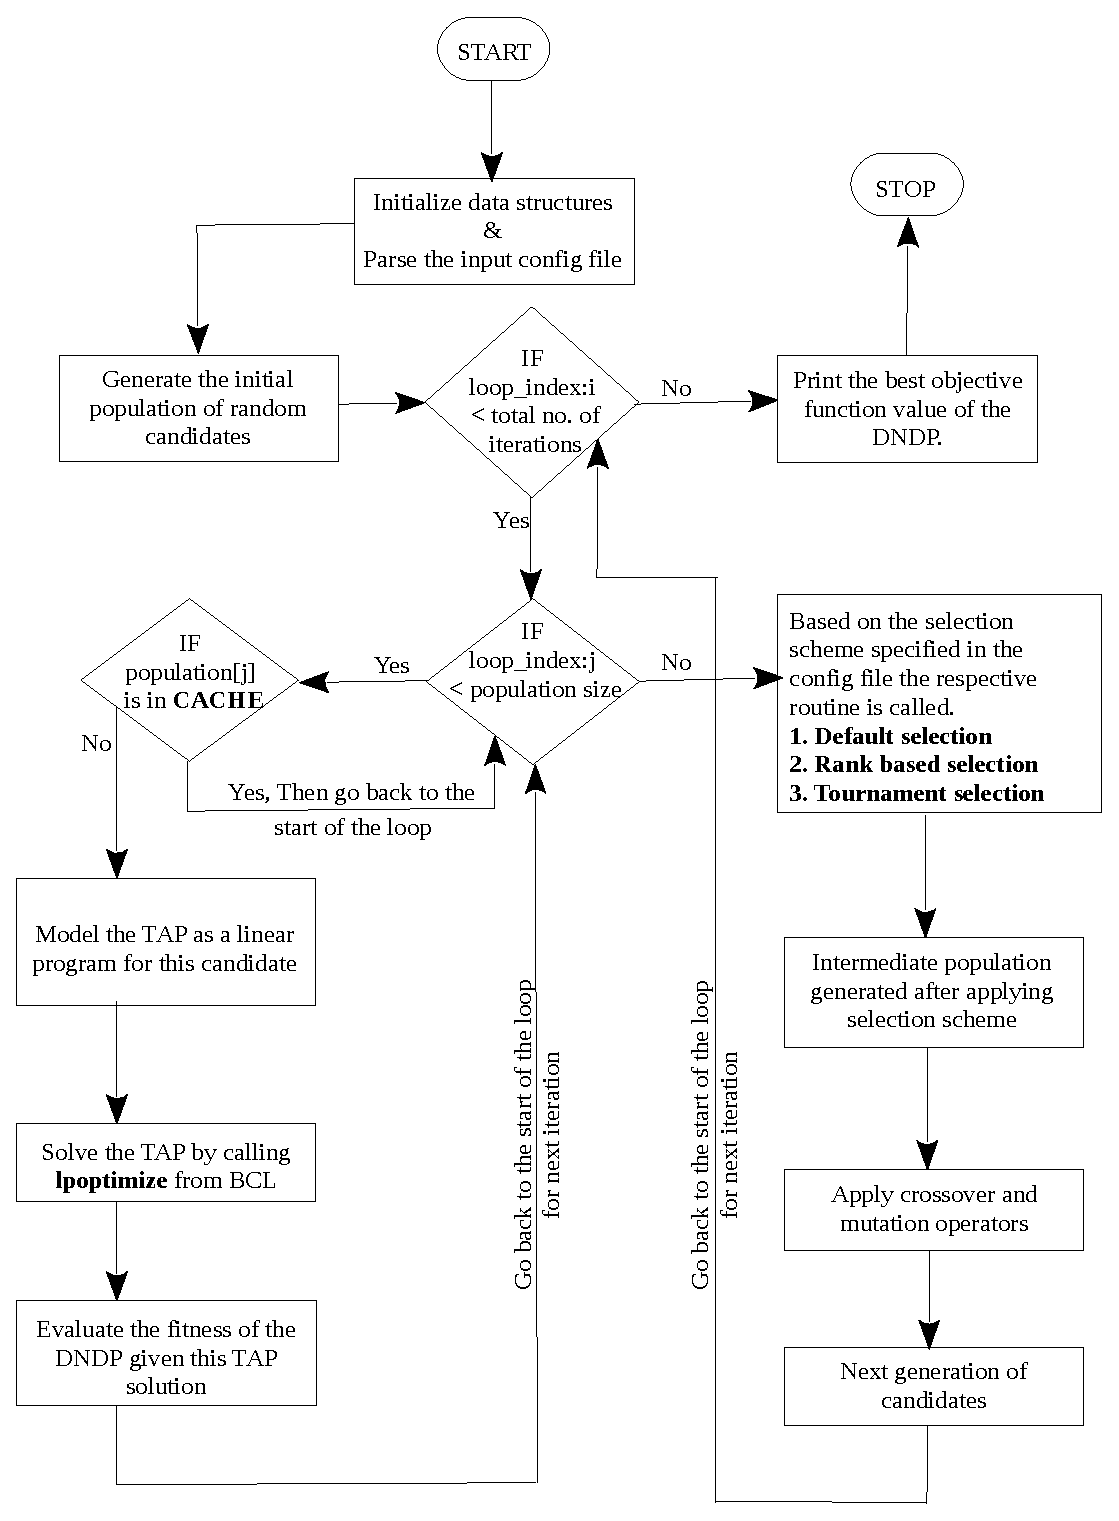
\includegraphics[scale=0.95]{./diagram.eps}%}
\caption{\textbf{Flow chart of the software imlementation}}
\label{fig 1}
\end{figure}
%}
%\end{minipage}[t]
%\afterpage{
%\thispagestyle{empty}
\begin{figure}[htbp]
\floatpagestyle{empty}
\hspace*{0.1in}
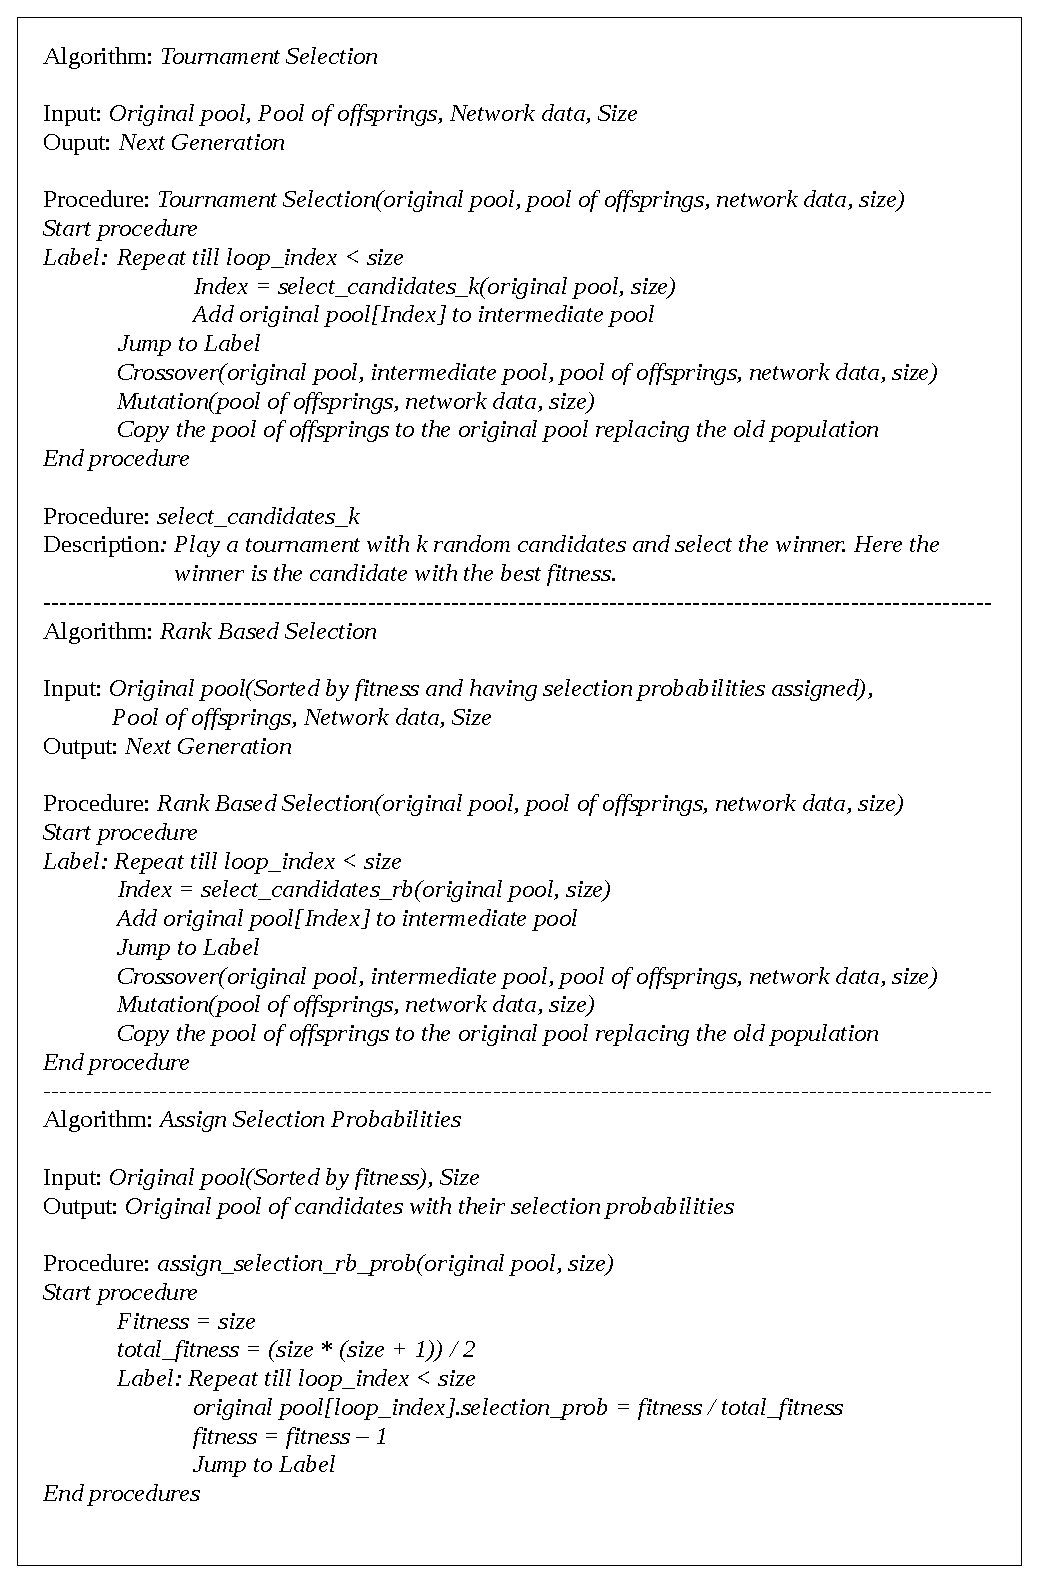
\includegraphics[scale=0.9]{./diagram1.eps}
\caption{\textbf{Pseudo code for algorithms}}
\label{fig 2}
\end{figure}
%}
%\afterpage{
%\thispagestyle{empty}
\begin{figure}[htbp]
\floatpagestyle{empty}
\hspace*{-0.10in}
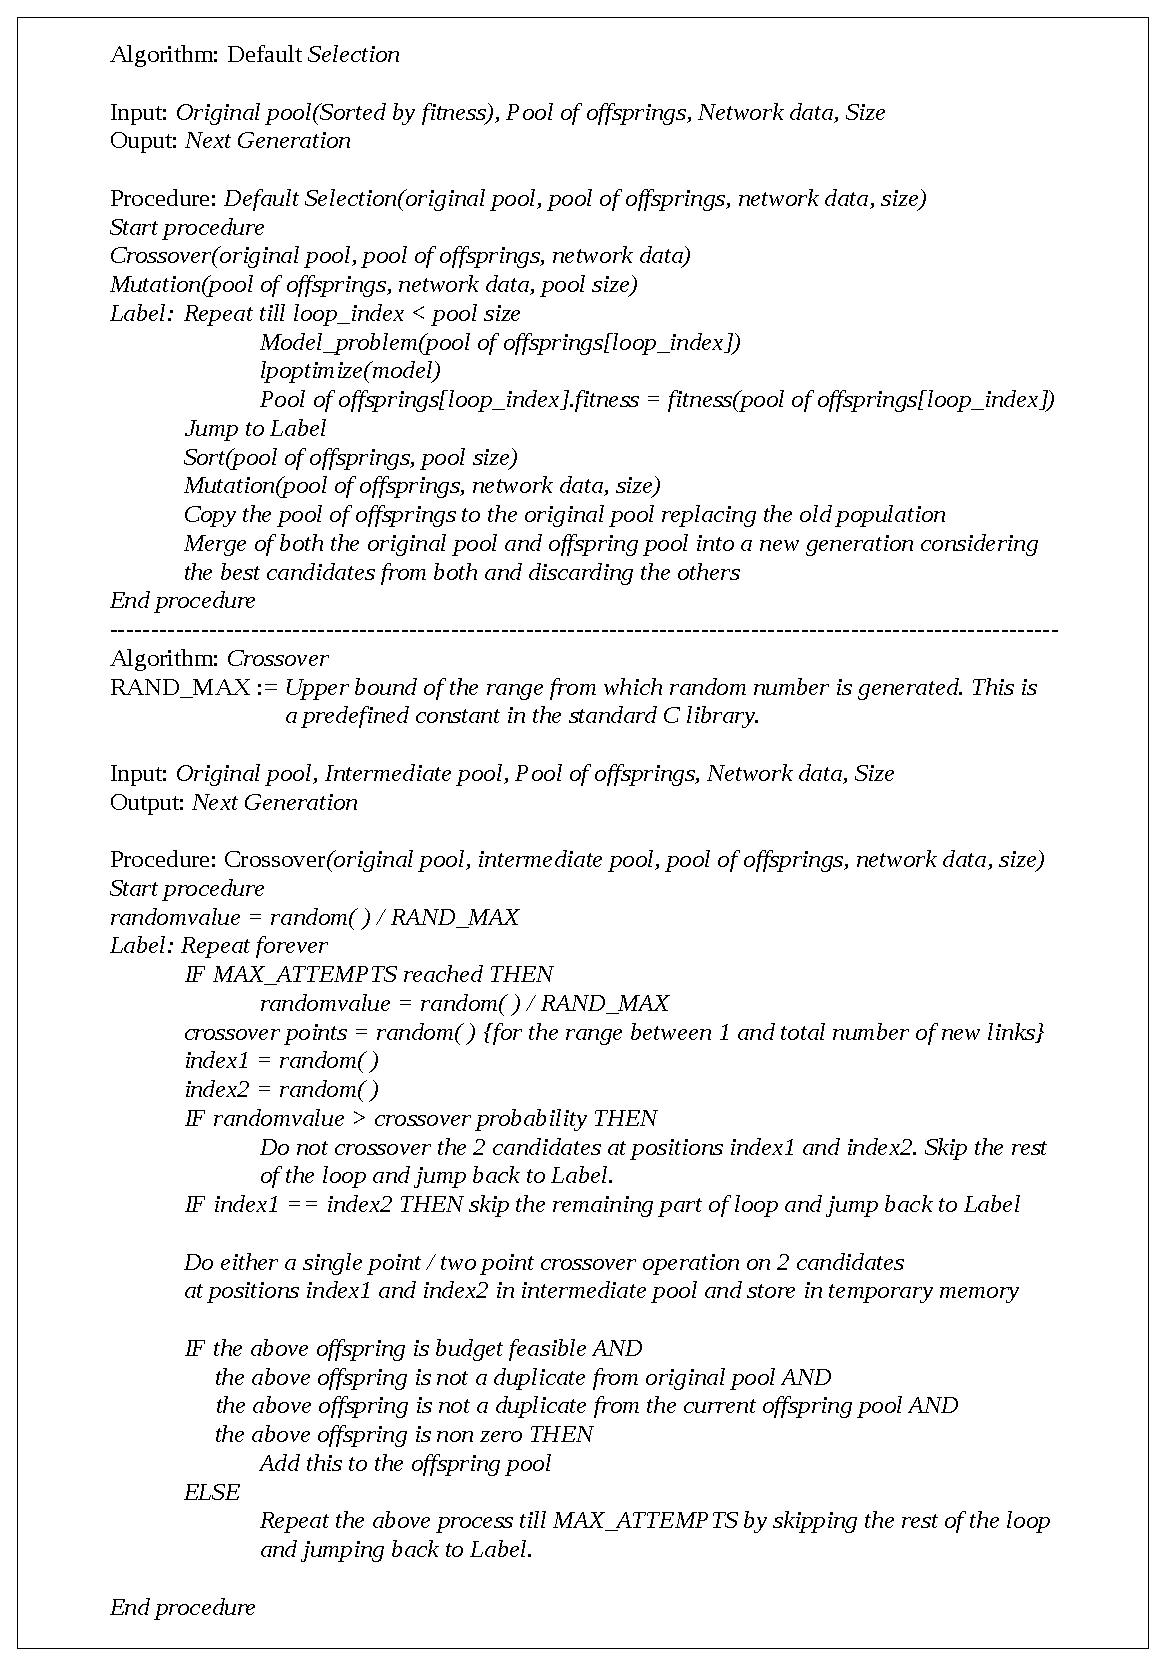
\includegraphics[scale=0.85]{./diagram2.eps}
\caption{\textbf{Pseudo code for algorithms}}
\label{fig 3}
\end{figure}
%}
\subsection{Software Design}
\subsection{Implementation Details}
\newpage
\section{Experiments and Visualization}
\subsection{Setup}
\subsection{Datasets}
\subsection{Experiments and Results}
\subsection{Visualization}
\newpage
\section{Conclusion}
\subsection{Scope for future work}
%\begin{figure}[h]
%\centering
%\includegraphics[width=0.65\textwidth, clip, trim=0mm 60mm 0mm 0mm]{data/architecture.pdf}
%\vspace{-0.15in}
%\caption{Invasive resource management architecture}
%\label{fig:arch}
%\end{figure}
\nocite{fontaine,gao,poorzahedy2,tianze,leblanc,kuo,poorzahedy1,wen}

\bibliographystyle{unsrt}
% Literature sources are to be found in seminarpaper.bib
\bibliography{nishanth}

\end{document}
